Large language models such as GPT-3~\citep{brown2020language} are able to perform \emph{in-context learning}:
given a prompt containing examples from a task (input-output pairs) and a new query input, the language model can generate the corresponding output.
For example, these models are able to produce English translations of French words after being prompted on a few  such translations, e.g.:
\[\underbrace{\ \text{maison} \to \text{house},\ \text{chat} \to \text{cat},\ \text{chien} \to \ }_\text{prompt}
\underbrace{\ \text{dog}\ }_\text{completion}.\]
This capability is quite intriguing as it allows models to adapt to a wide range of downstream tasks on-the-fly---i.e., without the need to perform any parameter updates after the model is trained~\citep{brown2020language,lieber2021jurassic, rae2021scaling, black2022gpt}.
However, it is unclear to what extent these models have developed the ability to learn \emph{new tasks} from in-context examples alone as opposed to simply indexing into a vast set of known tasks from the training data (e.g., see~\citet{min2022rethinking}).
% \footnote{Note that a more general notion of ``in-context learning''---which refers to any model behavior that utilizes information in the prompt to make predictions that improve with prompt size---has also been studied, e.g., see \citet{olsson2022context}.}
%\footnote{See \citet{olsson2022context} for other notions of in-context learning that we do not consider.}
% \footnote{The term ``in-context learning'' has also been used to refer to a more general notion of learning from the prompt, see~\citet{olsson2022context}. In this work, we focus on the notion which specifically refers to the few-shot learning of a task/function~\citep{brown2020language}.}
\footnote{The term ``in-context learning'' has also been used to refer to a more general notion of learning from a prompt~\citep{olsson2022context}. In this work, we focus on the standard notion which refers to learning a task/function given in-context examples~\citep{brown2020language}.}

To make progress towards understanding in-context learning, we consider the well-defined problem of learning a \emph{function class} from in-context examples.
%The goal of our work is to empirically understand in-context learning in a well-defined setting.
%Concretely, we frame in-context learning \pl{unclear why this is considered framing - we're talking about a different concept that's built on in-context learning of a fixed function} as the ability to learn a \emph{function class} from in-context examples.
That is, we say that a model can in-context learn a function class $\mathcal{F}$ if, for ``most'' functions $f \in \mathcal{F}$, the model can approximate $f(x_{\text{query}})$ for a new query input $x_{\text{query}}$ by conditioning on a prompt sequence $(x_1, f(x_1), \ldots,x_k, f(x_k), x_{\text{query}})$ containing in-context examples and the query input.

Formally, let $D_\mathcal{X}$ be a distribution over inputs and $D_{\mathcal{F}}$ be a distribution over functions in  $\mathcal{F}$. A prompt $P$ is a sequence $(x_1, f(x_1), \ldots, x_k, f(x_k), x_{\text{query}})$ where inputs (i.e., $x_i$ and $x_{\text{query}}$) are drawn i.i.d. from $D_\mathcal{X}$ and $f$ is drawn from $D_{\mathcal{F}}$. We say that a model $M$ can in-context learn the function class $\mathcal{F}$ up to $\epsilon$, with respect to  $(D_{\mathcal{F}}, D_\mathcal{X})$, if it can predict $f(x_\text{query})$ with an average error
\begin{equation}
\label{eq:in-context_loss}
\mathds{E}_{P}\left[\ell\left(M\left(P\right), f\left(x_{\text{query}}\right)\right) \right] \leq \epsilon,
\end{equation}
where $\ell(\cdot, \cdot)$ is some appropriate loss function, such as the squared error. 

Within this framework, we can now concretely ask: 
\begin{center}
    %\emph{What classes of functions can be in-context learned by a given model?}
    \emph{Can we train a model to in-context learn a certain function class?}
\end{center}
Note that, here, being able to in-context learn a function class is a property of model $M$ alone, independent of how it was trained.
\emph{Training} such a model can be viewed as an instance of \emph{meta-learning}~\citep{schmidhuber1987evolutionary, naik1992meta,thrun2012learning}, a general paradigm for learning a model or method that can learn from data.

We empirically study this question,  focusing on Transformer models~\citep{vaswani2017attention,radford2018improving}---the architecture behind recent large language models---trained from scratch to in-context learn a range of simple, well-defined function classes (e.g. linear functions).
Specifically, we sample prompts containing in-context examples (input-output pairs) generated using functions in a given class and train models to predict the function value at the corresponding query inputs. (see illustration in Figure~\ref{fig:setting}). Our findings are as follows.

\begin{figure}[htb]
    \centering
    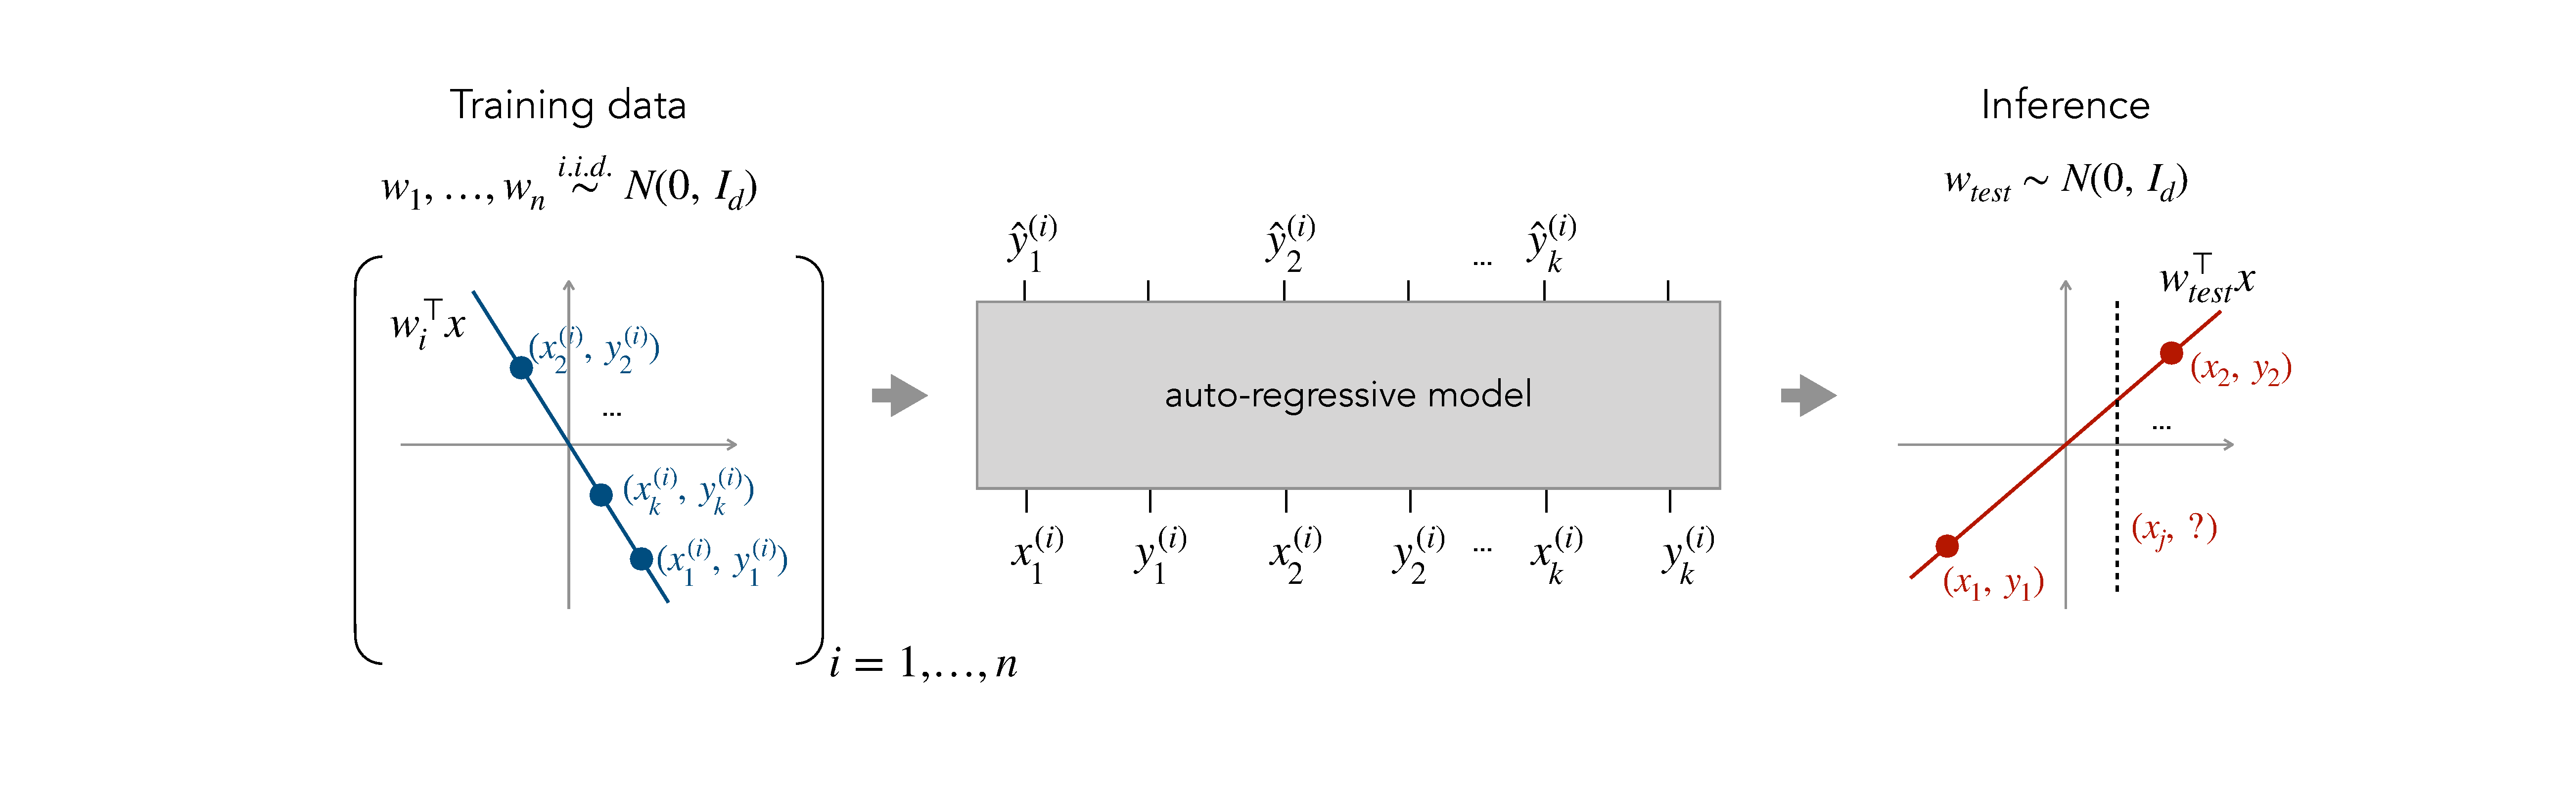
\includegraphics[width=\textwidth]{figures/setting.pdf}
    \caption{\emph{Can we train a model that in-context learns a function class (here linear functions)?}
    We train Transformers by repeatedly sampling a random function $f$ from that class, as well as random inputs $x_1, \ldots, x_k$ and training the model to predict each $f(x_i)$ given the prompt $x_1, f(x_1), \ldots , x_{i-1}, f(x_{i-1}), x_i$ (wrt squared loss).
    Then, during inference, we evaluate the model's ability to predict accurately on new, \emph{unseen} functions.
    }
    \label{fig:setting}
\end{figure}

%The focus of our work is on understanding whether we can efficiently train models \pl{confusing because we state that it doesn't depend on how it's trained, and now we sayy we're interested in training; maybe the main question should be: can we train a model to in-context learn a certain function class} to in-context learn a range of fundamental 
%\pl{fine to use this word, but use it eariler and consistently - before we're saying well-defined, simple, etc.}
% dt, we are using "well-defined in-context learning setting" and "fundamental function classes" so this is consistent
%function classes. We do this by sampling prompt sequences generated using functions in the class, and training the model from scratch on these sequences (see illustration in Figure~\ref{fig:setting}).
%We focus on Transformer models~\citep{vaswani2017attention,radford2018improving}---the architecture behind recent large language models.


\paragraph{Transformers can in-context learn linear functions.}
We show empirically that we can train a standard Transformer from scratch to in-context learn the class of linear functions, with respect to
the input distribution $D_{\mathcal{X}}$ being an isotropic Gaussian in 20 dimensions, and  $D_{\mathcal{F}}$ being the distribution over linear functions with weight vectors drawn from an isotropic Gaussian (the model was trained on prompts generated from the same distributions $D_{\mathcal{X}}$ and $D_{\mathcal{F}}$).
Specifically, the trained model achieves error comparable to the optimal least squares estimator, suggesting that it encodes an effective learning algorithm, at least for the distribution used to generate the training prompts.

\paragraph{Generalization to out-of-distribution prompts.}
To understand the extent to which the trained model encodes an algorithm that works beyond the training distribution, we consider in-context learning under two types of distribution shifts: (a) a shift between the prompts encountered during training and inference (e.g., training on prompts without any noise in the in-context example outputs but testing with noisy outputs), (b) a shift between the in-context examples and the query input during inference (e.g., in-context examples lie in one orthant and the query input lies in another). 
We find that the  performance of our model is quite robust to such shifts, indicating that it has learned to perform linear regression with some generality.

\paragraph{More complex function classes.}
We also consider the function classes of 3-sparse linear functions, two-layer ReLU neural networks with 100 hidden units, and decision trees of depth 4, all with 20 dimensional inputs.
We show that we can again train Transformer models that can in-context learn these classes (with respect to isotropic Gaussian inputs and appropriately defined distributions over functions). 
For sparse linear functions, the trained model is able to exploit sparsity, obtaining performance better than least squares and comparable to Lasso.
For neural networks, the corresponding model is able to obtain performance comparable to neural networks of the same architecture trained using gradient descent on in-context examples. Moreover, it is also able to in-context learn linear functions.
For decision trees, the trained model can learn unseen trees with as few as 100 in-context examples, whereas greedy learning and tree boosting algorithms are unable to achieve competitive performance (for the distribution of prompts studies here).
Note that learning these function classes requires involved algorithms (e.g., gradient descent with the Lasso objective), and our results show that Transformers can encode algorithms with similar performance in a single forward pass.

\paragraph{Role of model capacity and problem dimension.}
Finally, we explore how the ability of Transformers to in-context learn linear functions scales with model capacity and problem dimensionality. We find that increasing the capacity of the model improves performance significantly, and also allows the model to in-context learn higher-dimensional functions.
Moreover, increasing the capacity often significantly improves performance with distribution shifts, even when the absolute improvement in the standard error is small.